\chapter{Introduction to NoSQL Injection}
This section outlines the concept of NoSQL injection and how it derives from conventional SQL injection. A definition of NoSQL injection is given along with a detailed analysis of the corresponding attacker models.

\section{From SQL to NoSQL Injection}
\label{sec:fromSQLtoNoSQLinjection}
Injection attacks on relational databases represent the major web application vulnerability of the last decade \cite{OWASP:2013b}. Thereby, the three tier architecture composed of client, server and database plays an important role. Since data obtained from the client can be arbitrary manipulated, input validation and sanitizing represent important principles for the the server-side. Otherwise, unvalidated input may find its way into sensitive operations, that cause injection vulnerabilities. In case unvalidated data is used to build database queries, an attacker is able to alter the SQL statement's structure. Suchlike vulnerabilities represent serious threats, especially due to the direct data access in combination with the Touring completeness of the injected SQL context.\\ 

This situation changed with the emerging generation of NoSQL databases. A variety of new query techniques was introduced next to SQL. For many databases, JSON-based or parameterized function calls replaced the conventional SQL approach. These simplified methods lead to a more straightforward database access and enabled unstructured data models. All the same, program logic moved from the database to the application layer due to functional limitations of the queries. Complex operations, such as data constraints or checks, that were previously executed directly on the database with SQL, have to be implemented within the application layer. Bypassing these logical constraints in order to achieve a certain database behavior constitutes an important aspect in the context of NoSQL injection. \\ 

Beside the query techniques, also the architecture of systems diversified with the emerged NoSQL databases. Relational databases are similar regarding their strengths and weaknesses, leading to a deployment in typical system structures, like the three tier model. In contrast to that, NoSQL databases discern in their focused area of application. Special requirements demand for tailored databases or even a combination of them. This leads to heterogeneous system landscapes deploying different databases and technology stacks for distinct purposes. Data exchange between multiple databases becomes an vital aspect that has to be managed. The resulting diversity of system designs as well as the data exchange between different data models has to be considered for the attack surface of NoSQL injection. All in all, NoSQL injection faces a much more diverse environment in contrast to conventional SQL injection.

\section{Definition of NoSQL Injection}

In order to give a definition for injection attacks against NoSQL databases, multiple aspects have to be taken into account. The objective of an attack has to be clarified as well as the mightiness of an attacker. In the course of this, the varying system structures has to be considered. Thus, attacker models for NoSQL injection expose themselves much more diverse in comparison to conventional SQL injection. In general, NoSQL injection can be defined the following way:\\

\begin{description}
\item [NoSQL Injection] represents a class of attacks against non-relational databases, that cause unintended behavior of a query through insertion of malicious data into the query context. These vulnerabilities originate from unvalidated user input used as or as a part of a database query. Depending on the attacked database, the injected input is crafted with the aim to trigger unintended operations of the database layer affecting confidentiality, integrity or availability of data.
\end{description}

Similar to other classes of attacks, NoSQL injection is directed against at least one of the three security goals - confidentiality, integrity and availability. This class of attack is focused on the database layer of an application or more precisely the therein stored data. The attacker goal of NoSQL injection is to compromise this data with regard to any of the mentioned security goals. Unauthorized modification or retrieval of data as well as restriction of data access for others, represent successful attacks. These results can be achieved by triggering malicious query behavior, especially with regard to typical create, read, update and delete operations. Malicious behavior can be accomplished through manipulation of existing queries as well as the invocation of unauthorized queries. Bypasses for preceding confidentiality and integrity checks allow such query manipulation and invocation and constitute an important aspect for this class of attacks. User provided input in turn enables users as well as attackers to influence database queries. When data received from user input is not properly sanitized for the query context, an attacker might be able to manipulate the semantics and structure of the database operation. Inputs provided by users derive from requests received from clients. Since their content can be manipulated, these requests represent the attacker surface for NoSQL injection. Arbitrary manipulation is only limited by the fixed protocol structure used for the request. Otherwise, further processing of the request on the recipient side may fail. For an attack, a request with adapted contents is built, that leads to a database query with malicious user input. The database interprets the triggered query in a way that breaks one of the security goals for the underlying data. These circumstances define a successful NoSQL injection attack.\\

The given definition of NoSQL injection is described in a relatively generic way. This goes in accordance with the in section \ref{sec:fromSQLtoNoSQLinjection} elucidated diverse system environments. On account of these circumstances, the way user input takes until it reaches the database query distinguishes depending on the system environment. Therefore, the phase between attacker initiated request and actual invocation of a database operation faces different scenarios. To address this in scope of the NoSQL injection definition, the following sections analyze the most significant system scenarios and outline the according attacker models.

\subsection{Common Attacker Model}
\label{sec:commonAttackerModel}

When analyzing the potential system structures of the NoSQL environment, the three tier model still plays a major role. The combination of client, application server and database layer represents a fundamental structure for web applications. This architectural style builds the basis for the long known class of SQL injection attacks. Non-relational databases are also often deployed in the same way. Therefore, the common attacker model from SQL injection applies in a similar way for NoSQL injection attacks. An overview of the according attacker model including the involved data flows is illustrated in figure \ref{fig:normalAttackerModel}.

\begin{figure}[h]
\centering
  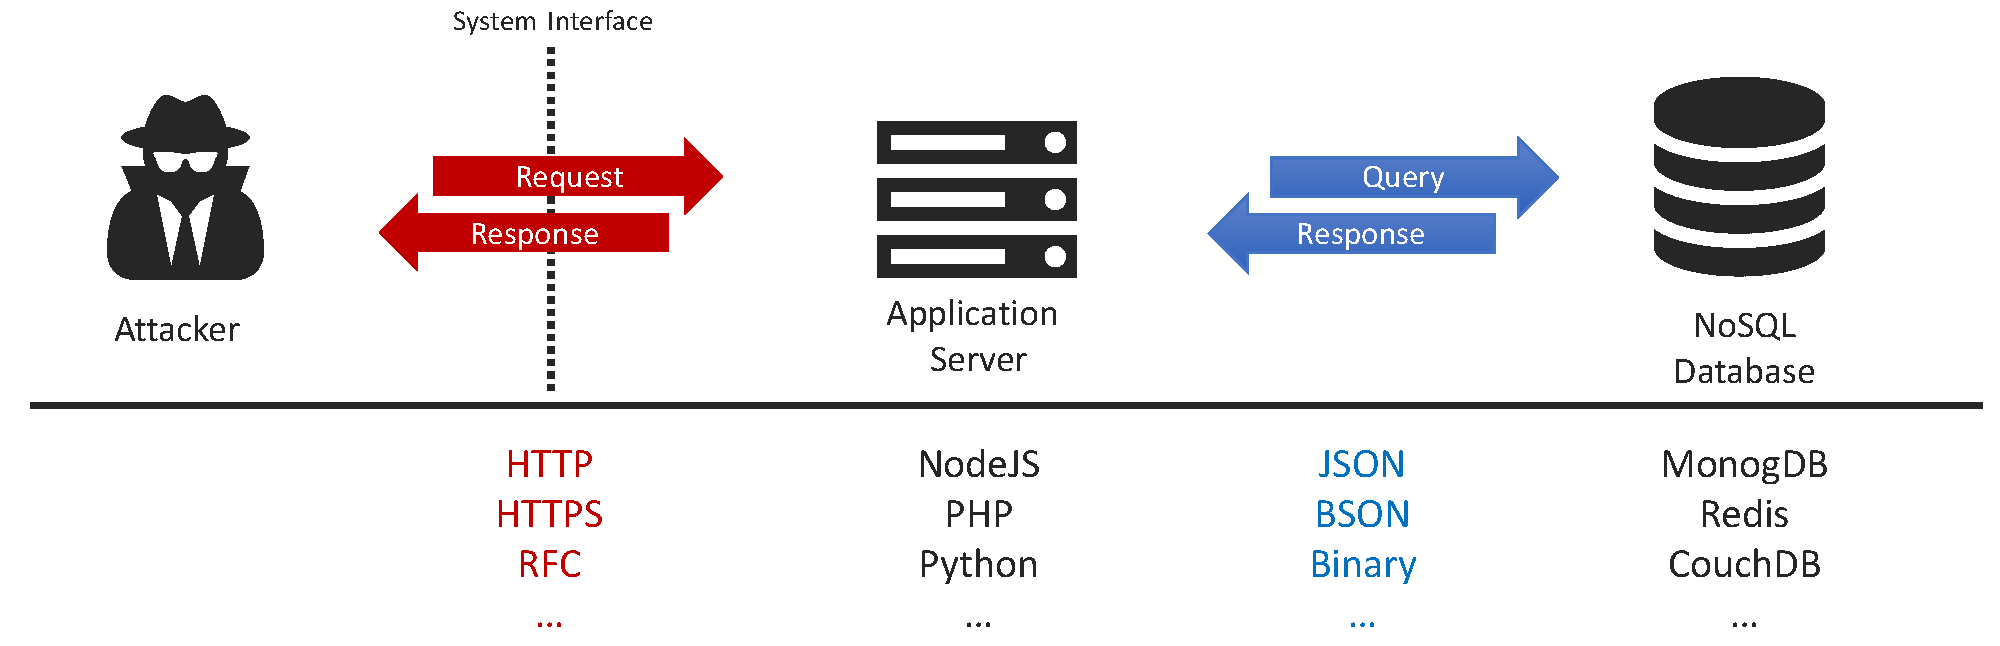
\includegraphics[width=1\linewidth]{Images/attacker_model_normal}
  \caption{Common attacker model for NoSQL injection}
  \label{fig:normalAttackerModel}
\end{figure}

The common attacker model can be described with a request-response cycle between the tree tiers. Initial requests of these cycles are normally originating from a client-side application. Since these client-side applications are under the control of individual users, requests sent to the application layer can be arbitrary manipulated and represent untrusted data. An attacker takes advantage of this and undertakes the role of a user or respectively the client-side application. The communication between client and server therefore represents the attacker surface and determines the scope for content manipulation. In order to initiate an attack, a request with the designated payload is crafted and sent to the application server. There, the received request containing malicious data is processed and becomes part of a database query. On the database layer, the manipulated query is interpreted and the results of this operation are returned to the application-layer. The resulting data is indirectly influenced by the doctored query, is passed through the response processing and delivered to the attacker in order to finish the request-response cycle. All processing steps mentioned in this cycle make changes to the data. When implemented securely, untrusted data is sanitized in these processing steps and injection attacks are prevented. Incomplete or even missing input sanitizing for the query context lead to potential NoSQL injection vulnerabilities.\\

\begin{minipage}[t]{0.48\textwidth}
  \textbf{Attacker Mightiness} \\ 
  The attacker is aware of the deployed tree tier technology stack including the utilized communication protocols, application platform and database. He is able to send arbitrary manipulated requests to the application server. Direct access to the NoSQL database layer for the attacker is not given.
\end{minipage}
\hfill
\begin{minipage}[t]{0.48\textwidth}
  \textbf{Attacker Goal} \\ 
  The attacker aims to achieve unintended behavior of at least one database query by altering its parameters. A successful attack compromises confidentiality, integrity or availability of the underlying data through the query processing step or the data received with the resulting response.
\end{minipage}

\subsection{Extended Attacker Model}

The emergence of NoSQL databases entailed diverse system structures and high data exchange between components as explained in section \ref{sec:fromSQLtoNoSQLinjection}. Multiple systems are deployed for different purposes and therefore exchange their data. As a consequence, data is transformed between different data models. A benign entry in one system may be critical in another one. An entry valid in one context, may result in a vulnerability when imported to another context. Therefore, data exchange becomes a critical aspect for interconnected systems. This situation has to be considered for determination of feasible attacker models. Figure \ref{fig:extendedAttackerModel} addresses suchlike environments and presents an extended attacker model. \\

\begin{figure}[h]
\centering
  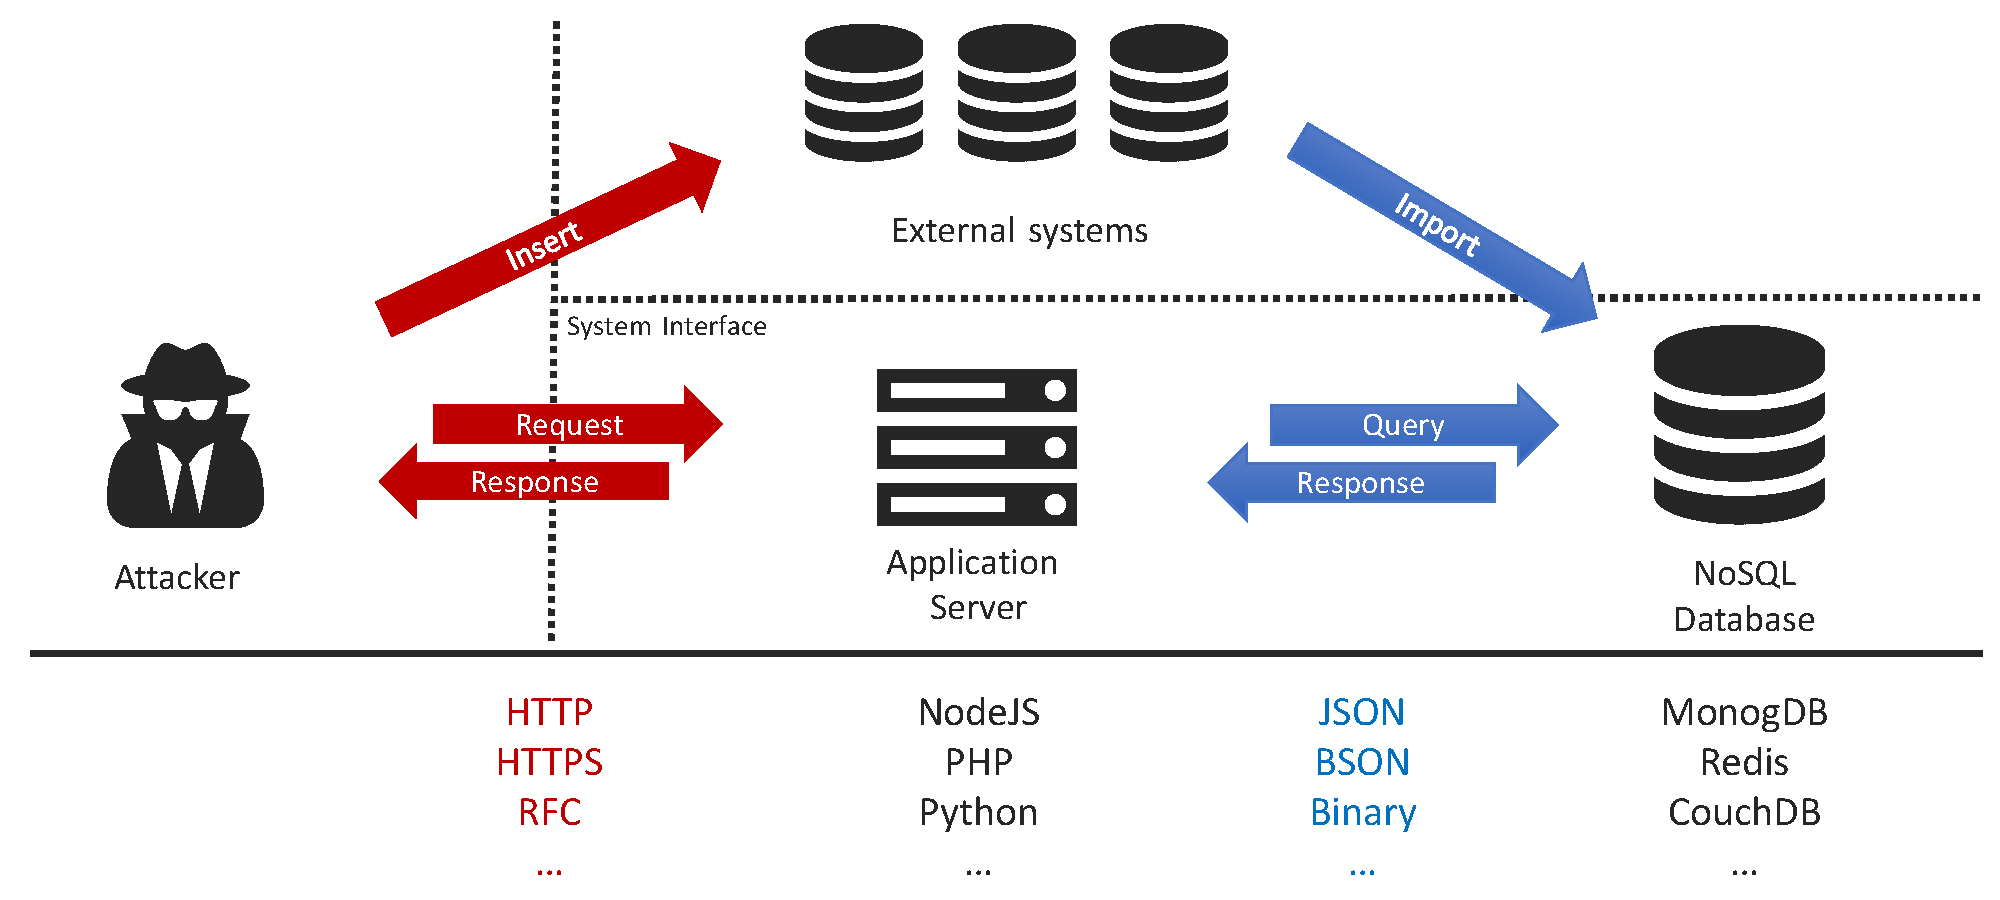
\includegraphics[width=1\linewidth]{Images/attacker_model_extended}
  \caption{Extended attacker model for NoSQL injection}
  \label{fig:extendedAttackerModel}
\end{figure}

This model extends the common attacker model described in section \ref{sec:commonAttackerModel} by a preceding step. NoSQL system circumstances do not necessarily allow the assumption, that the underlying data is completely tamper-proof. In this model, the database layer imports data from at least one external source. This source can be a file, another database or even an complete external system. The procedure of an attack begins with manipulated data added to this external source. It has to be clarified, that the added data can be totally eligible in this context. Any import of this data, into another system leads to a tampered data stock. The degree of attacker influence depends on the import processing, but in the worst case, the data is transfered one-to-one. This means, that such a preliminary step allows an attacker to add arbitrary manipulated records to the attacked database. In a second step the procedure of the common attacker model is executed. The question is, whether this extended model allows new kind of injection attacks not applicable for the common model. Certainly, the definition of attack mightiness and goal have to be adapted for the extended model as follows. \\

% 2-step approach
% assumption to be able to insert arbitrary data into a external system or further 
% attacker is able to insert arbitrary entry in database
% ATTACKER Mightiness + GOAL (- insert)

% Objective
\begin{minipage}[t]{0.48\textwidth}
  \textbf{Attacker Mightiness} \\ 
  The attacker is aware of the entire deployed technology stack including the utilized communication protocols, application platform, database and external data source. He is able to insert arbitrary manipulated data to the external source and send arbitrary manipulated requests to the application server. Direct access to the NoSQL database layer for the attacker is not given.
\end{minipage}
\hfill
\begin{minipage}[t]{0.48\textwidth}
  \textbf{Attacker Goal} \\ 
  The attacker aims to achieve unintended behavior of at least one database query by altering its parameters. A successful attack compromises confidentiality, integrity or availability of the underlying data, that not derived from the attacker. This can be achieve as a result of the import process, query processing step or the data received with the resulting response.
\end{minipage}


\subsection{Direct Attacker Model}
Another scenario that become important with NoSQL databases is direct communication between client and database layer. This is represented by a reduced three teer architecture, that does not deploy any application layer. The idea seems inconvenient, but is actually induced by multiple NoSQL databases. In contrast to the extended attacker model, also a simplified model is needed to address these kind of system structure. The two tier architecture and the corresponding attacker model are visualized within figure \ref{fig:directAttackerModel}.

\begin{figure}[h]
\centering
  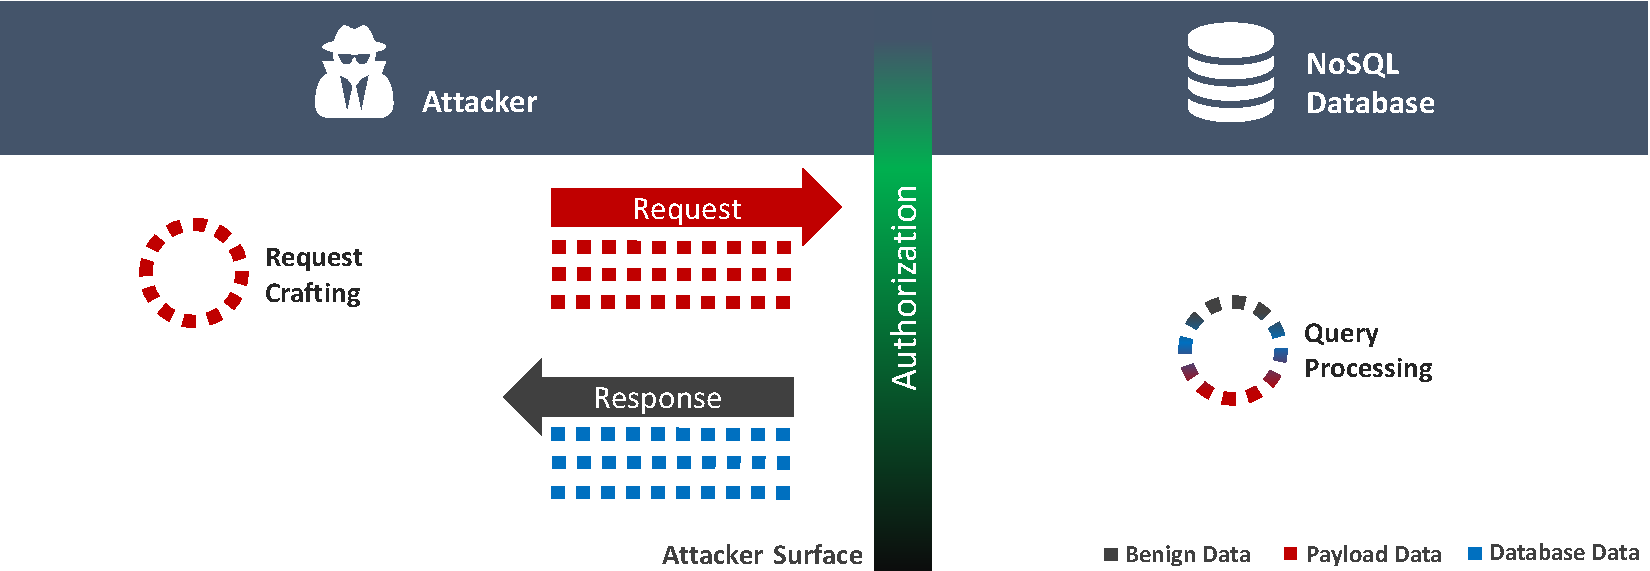
\includegraphics[width=1\linewidth]{Images/attacker_model_direct}
  \caption{Direct attacker model for NoSQL injection}
  \label{fig:directAttackerModel}
\end{figure}

The direct attacker model is based on a request-response cycle between client and database layer. Similar to the other models, the attacker overtakes the role of the client-side application and crafts a request containing the payload. This request is sent directly to the database layer. An important aspect of the entire attacker model is the authentication and authorization mechanism of the database. Otherwise, an attacker would be able to invoke arbitrary queries. In the scope of this model, the attacker is restricted by the authorization of an typical application user. At this point the granularity of the applied checks plays an important role. An successful attacker may craft a request, that passes the authorization checks and still triggers a potentially malicious behavior of the processed query. The major advantage for an attacker is that the manipulated request and resulting response are not processed, filtered or protected by any application layer. \\

\begin{minipage}[t]{0.48\textwidth}
  \textbf{Attacker Mightiness} \\ 
  The attacker is aware of the entire deployed technology stack including database layer, authorization checks and utilized communication protocol. He is able to send arbitrary manipulated requests directly to the database layer. This scenario implies direct access for the attacker to the attacked database with user-level authorization.
\end{minipage}
\hfill
\begin{minipage}[t]{0.48\textwidth}
  \textbf{Attacker Goal} \\ 
  The attacker aims to achieve unintended behavior the attacked database. A successful attack compromises confidentiality, integrity or availability of the underlying data through the query processing step or the data received with the resulting response.
\end{minipage}

\subsection{Combined Attacker Models}
With the previously outlined attacker models, the diverse scenarios for NoSQL-based systems are covered. The extended attacker model addresses the aspects of complex and unstructured data exchange between system components. With the direct attacker model the simplified two-tier architectures are taken into account. Due to the diverse system structures entailed by NoSQL databases, also combinations of these models become relevant in special cases. In comparison to the pretty uniform relational database environment, the definition of a holistic attacker model for the heterogeneous NoSQL environment is hard to ensure. Nevertheless, with the three presented attacker models, the most prevalent application structures of NoSQL databases are covered for the scope of this thesis. \\

By the detailed definition of NoSQL injection and the introduction of corresponding known as well as new attacker models, the in section \ref{sec:objective} set \textbf{Objective 1} is covered and the basis for the following elaboration is given.


\section{Considered Technology Stack}

The previously defined attacker models are held generic by not involving involve concrete databases, protocols or application servers. In this way, a holistic definition for NoSQL injection could be given. However, actual vulnerabilities and according attack vectors depend on designated technology configurations. With regard to the objective of NoSQL injection investigation, a scope for the considered technologies has to be set. An examination of all feasible technology combinations is not viable. This section selects the most prevalent technologies of each layer for the further investigation in scope of this thesis.

\subsection{Selected Databases}

The database layer constitutes a key aspect for the investigation of NoSQL injection. In order to provide a comprehensive exploration of the topic, the prevalence of the databases represents an important factor. The underlying data structures as well as query techniques have to be considered for a diverse selection, too. Especially databases, that implement concepts differing strongly form the well explored relational approach represent suitable candidates. As a basis for the selection, a ranking rating the popularity of databases was used. An extract of the top ranking non-relational databases is shown in table \ref{tab:db_ranking} \cite{Solid2016}.


\definecolor{light-gray}{rgb}{0.92,0.92,0.92}
\begin{table}[h]
 \sffamily 
 \centering
 \begin{tabular}{cllcc}
  \textbf{NoSQL Rank} & \textbf{Database} & \textbf{Type} & \textbf{Overall Rank} & \textbf{Trend} \\ \hline
  \rowcolor{light-gray} 1. &  MongoDB     & Document store & 4. & $\scriptstyle\nearrow$ \\
  2. &  Cassandra   & Column store & 7. & $\rightarrow$ \\
  \rowcolor{light-gray} 3. &  Redis       & Key-value store & 9. & $\scriptstyle\nearrow$ \\
  4. &  HBase       & Column store & 15. & $\rightarrow$ \\
  5. &  Neo4j       & Graph store & 21. & $\rightarrow$ \\
  6. &  Couchbase  & Document store & 22. & $\rightarrow$ \\
  \rowcolor{light-gray} 7. &  Memcached & Key-value store & 23. & $\rightarrow$ \\
  8. &  DynamoDB & Document store & 24. & $\scriptstyle\nearrow$ \\
  \rowcolor{light-gray} 9. &  CouchDB   & Document store & 27. & $\scriptstyle\searrow$ \\
  10. &  Riak KV & Key-value store & 32. & $\scriptstyle\searrow$ \\
  \bottomrule
 \end{tabular}
 \caption{Ranking of databases according to their popularity}
 \label{tab:db_ranking}
\end{table}

Listed are the ten most popular non-relational databases measured by a combination of search trends, social network and developer discussions as well as job offerings. Every entry contains the name of the database or more precisely the database management system, the type of the underlying data model, its overall rank considering relational databases and search engines and the popularity trend of the last month. 



% Why the others are slected for investigation, is outlined in the listing below

\begin{description}
\item [MongoDB] represents the prime non-relational database of the ranking and the trend indicates further growth. This document store challenges the leading relational databases and is therefore a suitable candidate for further investigation. 
\item [Redis] is the highest ranking key-value store and exhibits the uppermost growth rate of all listed NoSQL databases. Its growth is also reflected by the shown trend scores. With the in-memory stored key-value pairs, a new concept arrived in leading databases. These circumstances make Redis the second databases, considered for the scope of this work.
\item [Memcached] is another key-value store, but differs strongly from others like Redis. This database is optimized for any kind of caching on distributed systems. Data is only store temporarily and never persisted to disc. Due to the discrete approach of this database, is represents the third candidate for NoSQL injection examination.
\item [CouchDB] implements another document-store with an declining popularity trend. Since its concepts differs strongly from other document stores and builds the basis for multiple other non-relational databases, it still embodies an interesting database for the investigation of injection attacks.
\end{description}

The second ranking non-relational database Apache Cassandra and the fourth ranking HBase are not considered, since their querying techniques are based on SQL-like languages and prepared statements are offered as a secure injection mitigation technique. In case of the graph structured Neo4j data store, the same reasons apply. Concepts relatively close to the relational approach can probably secured with known techniques and are hence not addressed by this thesis. Couchbase is in large parts a fork of the selected CouchDB, implements an similar approach and therefore not taken into account. The main reason for the disregarding of DynamoDB is its proprietary nature as a part of Amazon web service products. Last of all, the Riak key-value store is not considered, because of its similar approach with Redis and declining popularity. With the selected four candidates for NoSQl injection investigation, a broad range of non-relational concepts is covered.


\subsection{Selected Application Platforms}
Next to the underlying database, a series of application platforms have to be selected regarding the common and the extended attacker model. An optimal choice would be application layers that are most frequently deploy in combination with the selected NoSQL databases. Unfortunately, representative statistics for suchlike cases are not available. Another option is the analysis of open-source applications with regard to the used programming language. GitHub's open repositories provide a broad range of projects, that allow an evaluation of a programming languages' popularity. Exactly this information was gathered and published by a GitHub engineer and builds the basis for the application layer selection for this thesis. The top ranking programming languages of more than a million analyzed public repositories are summarized in table \ref{tab:language_ranking} \cite{Zapponi2014}.

\begin{table}[h]
 \sffamily 
 \centering
 \begin{tabular}{clrr}
  \textbf{Rank} & \textbf{Repository Language} & \textbf{Active Repositories} & \textbf{Total Commits} \\ \hline
  \rowcolor{light-gray} 1. &  JavaScript     & 323,938 & 3,461,415 \\
  2. &  Java   & 222,852 & 2,323,315 \\
  \rowcolor{light-gray} 3. &  Python  & 164,852 & 1,654,226 \\
  4. &  CSS       & 164,585 & 1,810,013 \\
  \rowcolor{light-gray}5. &  PHP      & 138,771 & 1,391,467 \\
  \rowcolor{light-gray}6. &  Ruby  & 132,848 & 1,106,259 \\
   7. &  C\scriptsize\raisebox{.5ex}{++} & 86,505 & 1,013,761 \\
  8. &  C & 73,075 & 804,339 \\
  9. &  Shell   & 65,670 & 592,046 \\
  10. &  C\scriptsize\raisebox{.5ex}{\#} & 56,062 & 558,332 \\
  \bottomrule
 \end{tabular}
 \caption{Ranking of programming languages according to the number of public repositories on GitHub in 2014}
 \label{tab:language_ranking}
\end{table}
Listed are the ten most used repository languages of public projects along with the number of active repositories and the total of push commits. The reasons for the selection of the highlighted programming languages and the corresponding application layers are listed below.

\begin{description}
\item [NodeJS] represents the server-side execution environment of JavaScript. As shown in the ranking, JavaScript is by far the most used language in the analyzed open-source projects. The language is used within browsers on the client-side as well as for server-side applications. Many non-relational databases even allow direct scripting with this language. Therefore, JavaScript or respectively the server-side NodeJS is selected for further investigation.
\item [Python] is the third highest ranking programming language and known for its fast and easy prototyping abilities. Common use-cases represent server-side scripting and web development. Its characteristics make Python an essential application layer for the scope of this work.
\item [PHP] is the most widespread server-side application layer of web applications. That is reflected with the fifth place in the popularity ranking of programming languages. Since the typical deployment of PHP resembles the presented attacker models, the language is taken into account for the scope of this work.
\item [Ruby] is nearly as popular as PHP regarding the number of active repositories. In combination with the Rails framework, Ruby represents an established application layer for web applications. On this account Ruby is selected as the fourth application layer language for NoSQL injection investigation.
\end{description}

With the selected four application layers a broad realm for our attacker models is covered. The languages are part of many examples used for the introduction NoSQL databases. Despite its high ranking, Java is not considered for further investigation. This decision is based on the high number of Android repositories, that are not suitable for the presented attacker models. CSS was omitted, since it is no typical application language and only offers styling capabilities for websites.


\subsection{Selected Application Layer Protocols}
\label{sec:selectedAppLayerProtocols}

Through the selection of databases and application platforms, the applicable communications protocols are already entailed. The attacker models enable an attacker to send arbitrary manipulated requests. An important restriction at this point is, that the request has to be interpreted and the contained payload processed by the application or database layer. Therefore, protocol-breaking request are mostly discarded. Manipulation of requests is for this reason restricted to designated parts in practice. Theoretically any application layer protocol or even lower-level ones can be used for cross-layer communication. For the selected technology stacks, HTTP and HTTPS represents the relevant protocols regarding the attacker surface. The following list explains the components, that are predestinated for attacker manipulation. \\

\textbf{HTTP}\\
The HTTP protocol implements several methods indication the server-side operation type. These methods can be set by the attacker as well as the URI of the addressed resource. Especially, the query string of the URL or even the path are often used for parameterization of the server-side application. Cookies are passed as a header for custom data transfer and are also part of the attacker surface. Depending on the used method type, a request body section is included in the request. The data contained within the body is used to pass data from the client to the server or vice versa and therefore represents another suitable part for malicious modification. \\

\textbf{HTTPS}\\
HTTPS embodies a secured version of the HTTP protocol with transport level encryption. The actual format as well as the attacker surface is fairly equal to the one revealed by HTTP. Method, URL, Cookie as well as the body section represent the practical attacker surface. \\

In case of the body section, multiple data formats exist \cite{Freed1996a}. These are called MIME-types and state the kind of transfered data. Some of these are particularly relevant for the payload encoding and therefore the crafting of an attacker request. The three most common body data formats for application parameterization are explained in the following paragraphs \cite{Freed2016}.\\

\textbf{application/json} \\
This type indicates a string following the JSON syntax. These strings can be parsed by server or client and result in an object of the employed programming language. Objects exist of properties that can be multi-layered by referencing other objects. \\

\textbf{application/xml} \\
This type indicates a XML file. Similar to JSON, the file can be parsed by server or client and result in an object of the employed programming language. The XML format differs between properties and child elements and allows multi-layered structures.\\

\textbf{application/x-www-form-urlencoded} \\
This type indicates a string containing key-value pairs, that is encoded according to the query-string structure of an URL. Web forms use this encoding by default. Most application layers allow the automatic extraction of the received key-value pairs into an object.

\chapter{Approaching NoSQL Injection}
Before concrete injection vectors can be created, the employed query techniques of non-relational databases have to be examined. This chapter analysis possibilities to change the behavior of queries with user-controlled data. Therefore, the actual query interface is considered as well as the capabilities offered by the attacker surface.

\section{Analysis of Query Techniques}
\label{sec:analysisOfQueryTechniques}
In order to achieve behavioral changes of queries, their design has to be examined. The design involves some way to encode semantics and the semantics in turn define the resulting operations within the database layer. Unfortunately, there exists a variety of query techniques with different designs used for non-relational databases. Each technique works differently, but the basic means to specify a query's semantics can be broken down to a few approaches. In an attacker's perspective, a query can be seen as a set of parameters passed to the database layer. Therefore, the ways parameters encode semantic have to be analyzed. Basically, there exist three ways the semantic encoding for query parameters is accomplished for non-relational databases.\\

\textbf{Value Encoded} \\
The parameter's semantic is encoded through its value. Usually string parameters are used for this type of encoding, but other types are also feasible. The values follow a specific pattern, that indicates the operation to be performed. In the case of string values, often a special syntax is used in order to be interpreted within the database engine. An attacker can influence the query's behavior by altering the parameter's value. SQL injection exploits this kind of semantic encoding by altering the string values that are later-on interpreted by the database. Some databases discern between normal and special values of a parameter. Special values or ranges of values trigger other operations compared to normal values. This semantic encoding builds the foundation for the following ones and can be detected in nearly all query techniques.\\

\textbf{Type Encoded} \\
In addition to putting semantics into the value a parameter, also the data type can be used for semantic encoding. An passed string may trigger another operation than a passed integer. This demands for dynamic typing or overloading capabilities of the query interface. An attacker can influence the query's behavior by altering the parameter's data type.\\

\textbf{Object Structure Encoded} \\
On top the given value and type encoding, semantics can also be defined by a parameter's object structure. This is enabled by parameters composed of data types, such as objects and arrays, that in turn can contain further parameters. Thereby, nested objects structures are passed as a parameter to the database layer and operations are triggered depending on this structures. An attacker can influence the query's behavior by altering the parameter's object structure.\\

These are the three major means of non-relational databases to encode semantics into a query. Consequently, an attacker has to take influence on at least one of the three semantic encodings in order to compromise the targeted security goals.

\section{Analysis of Attacker Surface}
Based on the outlined approaches to alter query semantics, preceding steps of the attacker models have to be considered. The direct attacker model allows, as the naming implies, direct manipulation of the sent query parameters. In case of the common and the extend attacker model, the gap between attacker surface and query has to be bridged. Therefore, we take a deeper look at the application layer processing, its parameterization through parts of the HTTP request and how this can influence a query's semantic. Basically, we are searching for data flows originating from the attacker controlled request into a query invocation. As outlined within section \ref{sec:selectedAppLayerProtocols}, not all parts of a request are relevant in practice. Designated request parts are used for server-side application parameterization. These parts, known as request parameters, represent the sources of the required data flows. An attacker has to influence value, type or object structure of these request parameters before they reach the query invocation. Since requests and therefore the contained parameters are transfered to the application server as strings, only the value is manipulable without further processing. For type or object structure injection, some kind of interpretation has performed by the application layer. The following paragraphs analyze the injection possibilities of the selected request parameters for each of the investigated application platforms. \\

\textbf{Request URL - Path}\\
The URL determines the requested resource or called application and is composed of multiple sections. Two of these sections can be used for server-side application parameterization. The first one is the path declaration, that should actually define the directory of the requested file, but is often misused to pass string parameters. Its value is composed of strings separated by slashes. Since the path declaration is not further processed by any of the selected application layers, only the string contents can be adapted. This parameter is therefore limited to value manipulation of strings. In many cases, an adjusted path will result in rejected requests since the resource can no longer be found.\\ 

\begin{lstlisting}[escapechar=!, caption={Example for GET request}, label={lst:http_request_example}]
GET !\textbf{/path/to/resource}! HTTP/1.1
Host: example.org
\end{lstlisting}

\textbf{Request URL - Query String}\\
The second section of the URL, named query string, is much more common for application parameterization. The query string declaration is designed to pass key-value parameters to the server. By the official URL definition, this parameter is restricted to string values. One of the first published injection attacks on non-relational databases demonstrated, that PHP supports an extended query string syntax for object and array parameters \cite{Sullivan:2011}. The query string is parsed by default and the resulting objects are provided to the application. NodeJS does not include such functionality by default, but one of its packages does as another publication showed \cite{Petkov:2014a}. The article emphasized, that the concerned \textit{qs module} provides the same query string functionality and is used as a part of the major web server \textit{Express}. Listing \ref{lst:sqsyntax} gives an example for query strings that pass objects or respectively arrays to both platforms. \\

\begin{lstlisting}[caption={Examples for extended query string syntax}, label={lst:sqsyntax}]
?a[]=foo&a[]=bar // results in array ["foo", "bar"]
?a[foo]=bar      // results in object {foo : "bar"}
\end{lstlisting}

Further investigation in scope of this work showed, that the these features are much more widespread and powerful than revealed by previous publications. The object and array encoding syntax is supported by all major web servers across the selected application layers. On NodeJS the \textit{Express} web server is by far not the only one including the \textit{qs module}. Nearly every major web server implementation or REST client includes the \textit{qs module} and therefore supports the extended query string syntax. In addition, Ruby implements the same feature with the \textit{Rails} framework as well as Python does with its \textit{Django} framework. Thus, all notable web server implementations of the selected application platforms include this feature. Further, the syntax even allows the passing of nested objects and arrays as a parameter. Due to this non-standardized convenience functionality, the query string parameter enables an attacker to inject all necessary query string encodings. \\

\begin{lstlisting}[escapechar=!, caption={Example for GET request}, label={lst:http_request_example}]
GET /path/to/resource!\textbf{?foo=bar}! HTTP/1.1
Host: example.org
\end{lstlisting}

\textbf{Request Header - Cookies}\\
Within the header of each request a cookie parameter can be set. This cookie header is normally used for session handling between server and client or the tracking of your browser history, but can also be filled with any other data. Basically, the cookie parameter is a string that includes key-value pairs separated by semicolons. Depending on the application layer and applied framework, the entire cookie string or a parsed version is provided. Passing of objects, arrays or other types than strings is not natively supported on any of the observed platforms. Cookie strings therefore allow string value manipulation. \\

\begin{lstlisting}[escapechar=!, caption={Example for GET request}, label={lst:http_request_example}]
GET /path/to/resource HTTP/1.1
Host: example.org
Cookie: !\textbf{name=patrick; foo=bar}!
\end{lstlisting}

The request body is only used for specific HTTP methods, that transfer entire resources. Depending on the resource type, the format of the body content differs. In the context of NoSQL injection, three of these content types become particularly. \\

\textbf{Request Body - JSON}\\
As a standard data exchange format, JSON is also used as a data type for request bodies. JSON is specially relevant in the context of non-relational databases, because it is also an important storage format. By default, a JSON body is passed as a string to the application. In most cases, libraries are applied to parse the string into an equivalent object of the present language. This allows the encoding of values, types and object structures within the request body. \\

\begin{lstlisting}[escapechar=!, caption={Example for HTTP request}, label={lst:http_request_example}]
POST /path/to/resource HTTP/1.1
Host: example.org
Content-Type: !\textbf{application/json}!
Content-Length: 13

!\textbf{\{"user": "admin", "password": "1234"\}}!
\end{lstlisting}

\textbf{Request Body - XML}\\
XML represents another standard data exchange format, that can be applied to the body of a request. Similar to JSON, the XML is passed as a string to the application, but in most cases parsed by dedicated libraries. The resulting object of the present language describes the nodes and attributes of the XML document. This preset structure allows free manipulation of values, but data types and object structure are restricted by the node and attribute structure. In practice, this makes it hard to inject proper object structures.\\

\begin{lstlisting}[escapechar=!, caption={Example for HTTP request}, label={lst:http_request_example}]
POST /path/to/resource HTTP/1.1
Host: example.org
Content-Type: !\textbf{application/xml}!
Content-Length: 13

<?xml version="1.0" ?>
!\textbf{<data>}!
  !\textbf{<user>admin</user> }!
  !\textbf{<password>1234</password>}!
!\textbf{</data>}!
\end{lstlisting}

\textbf{Request Body - Form Data}\\
As the name applies, form data normally originates from web page forms. The format makes use of URL encoding or more specifically query string encoding. By definition, it allows simple key-value pairs. Since in most cases the same preprocessing as for normal query strings is applied, the extended syntax can be applied for this body format. This allows the definition of values, types as well as object structures that are parsed into the according application layer language.\\

\begin{lstlisting}[escapechar=!, caption={Example for HTTP request}, label={lst:http_request_example}]
POST /path/to/resource HTTP/1.1
Host: example.org
Content-Type: !\textbf{application/x-www-form-urlencoded}!
Content-Length: 13

!\textbf{user=admin\&password=1234}!
\end{lstlisting}

Across all investigated platforms, the parameters allow similar injection capabilities for the three semantic encoding styles. The results are summarized int table \ref{tab:request_parameter}.

\begin{table}[h]
  \sffamily
  \centering 
  \begin{tabular}{llcccl}
  \multirow{2}{*}{\textbf{Parameter}} & \multirow{2}{*}{\textbf{Format}} & \multicolumn{3}{c}{\textbf{Encoding}} \\
    & & \textbf{Value} & \textbf{Type} & \textbf{Structure} \\ \hline
  \multirow{2}{*}{URL}
    & Path & \cmark & \xmark & \xmark \\
    & \cellcolor{light-gray}Query string & \cellcolor{light-gray}\cmark & \cellcolor{light-gray}\cmark & \cellcolor{light-gray}\cmark \\ \hline
  Header & Cookie & \cmark & \xmark & \xmark \\ \hline
  \multirow{3}{*}{Body}
    & \cellcolor{light-gray}application/json & \cellcolor{light-gray}\cmark & \cellcolor{light-gray}\cmark & \cellcolor{light-gray}\cmark \\
    & application/xml & \cmark & (\cmark) & (\cmark) \\ 
    & \cellcolor{light-gray}application/x-www-form-urlencoded & \cellcolor{light-gray}\cmark & \cellcolor{light-gray}\cmark & \cellcolor{light-gray}\cmark \\ \hline
  \end{tabular}
  \caption{Interpretation of request data through application layer processing across the investigated platforms}
  \label{tab:request_parameter}
\end{table}

Highlighted are the three parameter formats, that enable an attacker to inject manipulated values, types and object structures into the application layer. Especially convenience functionalities for the query string and from data that are not officially standardized offer great opportunities for NoSQL injection vectors.

